\documentclass[openany]{article}

%Typesetting and language
\usepackage[american]{babel}
\usepackage[T1]{fontenc}
\usepackage{charter}
\usepackage{enumitem}
\usepackage{hyperref}

%Symbols
\usepackage{amssymb, amsmath, amsthm, bm}
\usepackage{mathrsfs}
\usepackage{mathtools}
\usepackage{marvosym}
\usepackage{MnSymbol}

%Colors & graphics
\usepackage[dvipsnames]{xcolor}
\usepackage{pgfplots}
\usepackage[numbered,framed]{matlab-prettifier}
\usepackage{pgfplots}
\usepackage{listings}
\usepackage{tikz}
\usetikzlibrary{arrows.meta}
\usepackage[object=vectorian]{pgfornament}
\usepackage{wrapfig}
\usepackage{varwidth}
\usepackage[framemethod=TikZ]{mdframed}
\usepackage{caption}
\usepackage{float}
\usepackage{geometry}
\usepackage{ulem}
\usepackage[most]{tcolorbox}
\usepackage{array}

\setlength{\parindent}{0pt}

\makeatletter
\g@addto@macro\bfseries{\boldmath}
\makeatother


\renewcommand{\Re}{\mathfrak{Re}}
\renewcommand{\Im}{\mathfrak{Im}}

\geometry{left=2cm,right=2cm,bottom=2cm,top=2cm}

\usepackage{fancyhdr}
\pagestyle{fancy}
\fancyhf{}
\renewcommand{\sectionmark}[1]{\markright{\arabic{section} - #1}}
\cfoot{\thepage}
\lhead{CS270}
\chead{HW10}
\rhead{Adam Yang}
\renewcommand{\headrulewidth}{1pt}


\DeclareMathOperator{\sgn}{sgn}
\DeclareMathOperator{\im}{im}
\DeclareMathOperator{\var}{var}
\DeclareMathOperator{\Orb}{Orb}
\DeclareMathOperator{\Fix}{Fix}
\DeclareMathOperator{\Stab}{Stab}
\DeclareMathOperator{\cov}{cov}
\DeclareMathOperator*{\esssup}{ess\,sup}
\DeclareMathOperator{\corr}{corr}
\DeclareMathOperator{\lik}{lik}
\DeclareMathOperator*{\argmin}{argmin}
\DeclareMathOperator*{\argmax}{argmax}

\newcommand{\niceline}[2]{%
		\nointerlineskip \vspace{.5\baselineskip}\hspace{\fill}
		{\color{#1}
				\resizebox{0.5\linewidth}{2ex}
				{{%
								{\begin{tikzpicture}
										\node  (C) at (0,0) {};
										\node (D) at (9,0) {};
										\path (C) to [ornament=#2] (D);
										\end{tikzpicture}}}}}%
		\hspace{\fill}
		\par\nointerlineskip \vspace{.5\baselineskip}
}

\definecolor{darkViolet}{HTML}{9400D3}
\newcommand{\sweetline}{%
		\noindent
		\begin{center}
				{\color{darkViolet}
						\resizebox{0.5\linewidth}{1ex}
						{{%
										{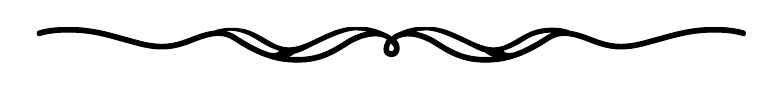
\begin{tikzpicture}
												\node  (C) at (0,0) {};
												\node (D) at (9,0) {};
												\path (C) to [ornament=85] (D);
												\end{tikzpicture}}}}}%
		\end{center}
}

\definecolor{remarkPurple}{HTML}{8346FF}
\definecolor{defBlue}{HTML}{0673FF}
\definecolor{exPurple}{HTML}{FF8710}

%THEOREM
\newtcbtheorem[auto counter,number within=section]{theorem}{Theorem}%
{enhanced,colback=white, breakable,frame empty,interior empty,colframe=cyan!50!white, top=8mm,
				coltitle=black,fonttitle=\bfseries,colbacktitle=cyan!15!white,
				borderline={0.5mm}{0mm}{cyan!15!white},
				borderline={0.5mm}{0mm}{cyan!50!white,dashed},
				attach boxed title to top left={yshift=-4mm},
				boxed title style={sharp corners=east,boxrule=1pt},varwidth boxed title}{thm}

%PROPOSITION
\newtcbtheorem[use counter from=theorem]{proposition}{Proposition}%
{enhanced,colback=white,breakable,frame empty,interior empty,colframe=defBlue!75!white, top=8mm,
				coltitle=black,fonttitle=\bfseries,colbacktitle=defBlue!20!white,
				borderline={0.5mm}{0mm}{defBlue!20!white},
				borderline={0.5mm}{0mm}{defBlue!50!white,dashed},
				attach boxed title to top left={yshift=-4mm},
				boxed title style={sharp corners=east,boxrule=1pt},varwidth boxed title}{prop}

%DEFINITION
\newtcbtheorem[use counter from=theorem]{definition}{Definition}%
{enhanced,colback=white,breakable,frame empty,interior empty,colframe=defBlue!75!white, top=8mm,
				coltitle=black,fonttitle=\bfseries,colbacktitle=defBlue!20!white,
				borderline={0.5mm}{0mm}{defBlue!20!white},
				borderline={0.5mm}{0mm}{defBlue!50!white,dashed},
				attach boxed title to top left={yshift=-4mm},
				boxed title style={sharp corners=east,boxrule=1pt},varwidth boxed title}{def}

%COROLLARY
\newtcbtheorem[use counter from=theorem]{corollary}{Corollary}%
{enhanced,colback=white,breakable,frame empty,interior empty,colframe=defBlue!75!white, top=8mm,
				coltitle=black,fonttitle=\bfseries,colbacktitle=defBlue!20!white,
				borderline={0.5mm}{0mm}{defBlue!20!white},
				borderline={0.5mm}{0mm}{defBlue!50!white,dashed},
				attach boxed title to top left={yshift=-4mm},
				boxed title style={sharp corners=east,boxrule=1pt},varwidth boxed title}{cor}

%REMARK
\newtcbtheorem[no counter]{remark}{Remark}%
{detach title, colback=white,enhanced ,breakable,frame empty, interior empty, fonttitle=\bfseries, coltitle=Violet, before upper={\tcbtitle.\quad},
				borderline west={0.5mm}{0mm}{remarkPurple!40!white},
				borderline west={0.5mm}{0mm}{remarkPurple!60!white,dashed}}{remark}

%LEMMA
\makeatletter
\newtcbtheorem[number within = tcb@cnt@theorem]{lemma}{Lemma}%
{enhanced,breakable,colback=white,frame empty,interior empty,colframe=orange!75!white, top=8mm,
				coltitle=black,fonttitle=\bfseries,colbacktitle=orange!20!white,
				borderline={0.5mm}{0mm}{orange!20!white},
				borderline={0.5mm}{0mm}{orange!50!white,dashed},
				attach boxed title to top left={yshift=-4mm},
				boxed title style={sharp corners=east,boxrule=1pt},varwidth boxed title}{lemma}
\makeatother


%PROOF
%%{enhanced,breakable,frame empty,interior empty,colframe=remarkPurple!75!white, top=8mm,
%	coltitle=black,fonttitle=\bfseries,colbacktitle=remarkPurple!20!white,
%	borderline={0.5mm}{0mm}{remarkPurple!20!white},
%	borderline={0.5mm}{0mm}{remarkPurple!50!white,dashed},
%	attach boxed title to top left={yshift=-4mm},
%	boxed title style={sharp corners=east,boxrule=1pt},varwidth boxed title}{prf}


\tcolorboxenvironment{proof}{% amsthm' 
				blanker,breakable,left=5mm,
				before skip=10pt,after skip=10pt,
				borderline west={0.5mm}{0pt}{cyan!40},
				borderline west={0.5mm}{0pt}{remarkPurple!10, dashed}}

%PROBLEM
\newtcbtheorem[auto counter]{problem}{Problem}%
{enhanced,breakable,colback=white,frame empty,interior empty,colframe=cyan!50!white, top=8mm,
				coltitle=black,fonttitle=\bfseries,colbacktitle=cyan!20!white,
				borderline={0.5mm}{0mm}{cyan!20!white},
				borderline={0.5mm}{0mm}{cyan!50!white,dashed},
				attach boxed title to top left={yshift=-4mm},
				boxed title style={sharp corners=east,boxrule=1pt},varwidth boxed title}{prob}

%EXAMPLE
%\newtcbtheorem[use counter from=problem]{example}{Example}%
%{enhanced,breakable,colback=white,frame empty,interior empty,colframe=remarkPurple!50!white, top=8mm,
%		coltitle=black,fonttitle=\bfseries,colbacktitle=remarkPurple!30!white,
%		borderline={0.5mm}{0mm}{remarkPurple!30!white},
%		borderline={0.5mm}{0mm}{remarkPurple!30!white,dashed},
%		attach boxed title to top left={yshift=-4mm},
%		boxed title style={sharp corners=east,boxrule=1pt},varwidth boxed title}{ex}


\newtcbtheorem[use counter from=theorem]{example}{Example}%
{detach title, colback=white,enhanced ,breakable,frame empty, interior empty, fonttitle=\bfseries, coltitle=black, before upper={\tcbtitle.\quad},
		borderline west={0.5mm}{0mm}{remarkPurple!30!white},
		borderline ={0.5mm}{0mm}{remarkPurple!30!white}}{example}

%SOLUTION
\newtcbtheorem[no counter]{solution}{Solution}%
{enhanced,breakable,colback=white,frame empty,interior empty,colframe=green!75!white, top=8mm,
				coltitle=black,fonttitle=\bfseries,colbacktitle=green!20!white,
				borderline={0.5mm}{0mm}{green!20!white},
				borderline={0.5mm}{0mm}{green!50!white,dashed},
				attach boxed title to top left={yshift=-4mm},
				boxed title style={sharp corners=east,boxrule=1pt},varwidth boxed title}{sol}
\definecolor{realPurple}{HTML}{AA05F9}
\definecolor{gray}{rgb}{0.5,0.5,0.5}
\definecolor{dkgreen}{rgb}{0,0.6,0}
\definecolor{mauve}{rgb}{0.58,0,0.82}

\lstset{frame=tb,
				style=Matlab-editor,
				language=C,
				aboveskip=3mm,
				belowskip=3mm,
				xleftmargin=3mm,
				showstringspaces=false,
				columns=flexible,
				frame=none,
				basicstyle={\small\ttfamily},
				numberstyle=\tiny\color{gray},
				keywordstyle=\color{blue},
				commentstyle=\color{dkgreen},
				stringstyle=\color{mauve},
				breaklines=true,
				breakatwhitespace=true,
				mlshowsectionrules = true,
				tabsize=3,
                    escapechar = ~,
				backgroundcolor=\color{cyan!5}
}

\newcommand\mmybox[2][fill=cyan!20]{%
    \tikz[baseline]\node[%
        inner ysep=0pt, 
        inner xsep=2pt, 
        anchor=text, 
        rectangle, 
        rounded corners=1mm,
        #1] {\strut#2};%
}


\def\changemargin#1#2{\list{}{\rightmargin#2\leftmargin#1}\item[]}
\let\endchangemargin=\endlist

\linespread{1.4}



% MAIN DOC
\begin{document}

\title{HW 10}
\author{Adam Yang}
% \date{\today}
\maketitle




\section*{Problem1}

\begin{proof}[Decision Problem]
    \renewcommand{\qedsymbol}{}
    
    Given a graph $G=(V,E)$ with $n$ nodes and $m$ edges, where the nodes are the enclosures, and the edges capture proximity. Given $k_M \geqslant 0$ male lions and $k_F\geqslant 0$ female lions, each with \textit{territoriality} $t_i \geqslant 0$ (integer). When lion $i$ is connected with another lion in same gender, $i$ will create \textit{territoriality} $t_i$. Is there a way to assign lions to make the total \textit{territoriality} at most $T$ and each enclosure has at most one lion?
    
\end{proof}

\begin{proof}{NP}

\textbf{Certificate:} A proposed assignment $k_M$ male lions and $k_F$ female lions to $n$ enclosures, each with $t_i$ territoriality.

\textbf{Certifier:} 
1. For each vertex (enclosure), check if there is at most one lion.

2. Let $T'$ denote the total territoriality in the proposed assignment, initialized to $0$. For each vertex $i$ (enclosure), add $t_i$ to $T'$ if $i$ has sex trouble (adjacent with same sex). If $T' \leqslant T$, then "YES", else then "NO". 

\textbf{Polynomial Runtime:} Certifier takes polynomial time for looping through all $|V|$ nodes and $|E|$ edges, thus $\mathcal{O}(m+n)$. Thus, it is a NP problem.
\end{proof}

\qquad \textbf{For convenience, name the problem as TERRITORIALITY.}

\begin{proof}{NP-Complete}



\textbf{Goal:} By proving INDEPENDENT-SET $\leqslant_p$ TERRITORIALITY, we can prove that this problem is a NP-hard and thus NP-complete problem. (NP proved above)

\textbf{Reduction Function:} Denote the reduction function as $f$. The input to $f$ is input to INDEPENDENT-SET (a graph $G$ and integer $k$), the output of $f$ is the input to TERRITORIALITY (a graph $G'$, $k_M$, $k_F$, $t_i$, and $T$). "YES" instance to INDEPENDENT-SET maps to "YES" instance to TERRITORIALITY, "NO" to "NO". 

\textbf{Reduction:} Set $G' = G$, $k_M$ or $k_F$ to $0$. WLOG(either male to 0 or female to 0 works), set $k_F=0$, $k_M = k$. For each lion $i$, set \textit{territoriality} $t_i=\infty$. Set $T=0$. 

\textbf{Proof of reduction:}

\qquad \textbf{Polynomial Reduction:} The reduction only renames and declares new parameters needed in TERRITORIALITY, therefor it's polynomial.

\qquad \textbf{"YES" to "YES":} By definition, $G$ has an independent set of size at least $k$ $\Rightarrow$ there are at least $k$ disjoint nodes in $G$. Since $G' = G$, if there are at least $k$ disjoint nodes, TERRITORIALITY will output "YES" by assigning all $k_M$ lions to the corresponding disjoint nodes (no two male lions will be adjacent to each other and thus no $t_i$ generated, $T=0$).

\qquad \textbf{"NO" to "NO":} (contrapositive) If there is a way to assign $k$ male lions to $G$ with $T=0$, then these $k$ lions are assigned in disjoint enclosures. Each enclosure is a node, therefore, these enclosures is a satisfying independent set with size $k$. [Direct proof is also easy: if there exists there are some adjacent nodes in the proposed set of nodes ("NO" for INDEPENDENT-SET), then there must be some adjacent enclosures, thus $T>0$ ("NO" for territoriality)]


\qquad Now that TERRITORIALITY is NP and NP-Hard, it is NP-Complete.

\end{proof}

\section*{Problem2}

\begin{proof}[Decision Problem]
    \renewcommand{\qedsymbol}{}
    $n$ guests. For each guest $i$, you are given three integers $h_i, s_i, f_i$. This means that guest $i$ will be available to hug during the time interval $[s_i, f_i]$. You want to hug them for $h_i \geqslant 0$ time. You can hug only one person at a time, and no hugs can be resumed/interrupted.
    Is there a way to hug everyone for the desired amount of time?
\end{proof}

\begin{proof}{NP}

\textbf{Certificate:} A proposed assignment to hug everyone with start time $t_i$ to start hugging each guest $i$.

\textbf{Certifier:} 1. Check if the size of assignment is $n$. If the size is less than $n$, then "NO" because we can't hug everyone one.

2. Check if $\forall t_i: [t_i, t_i+h_i]$ lies within $[s_i, f_i]$.

3. Check if no two hugging time $[t_i, t_i+h_i]$ and $[t_j, t_j+h_j]$ are overlapped $(t_i \neq t_j)$.

\textbf{Polynomial Runtime:} Certifier is polynomial for looping through all $n$ guests, $\mathcal{O}(n)$. 

Thus, THANKSGIVING-HUG is NP problem.

\end{proof}

\begin{proof}{NP-Hard}

\textbf{Note:} SUBSET-SUM will be defined just as discussed in discussion session: Given a set $C$ of $n$ natural numbers, is there a subset of $C$ S.T. its sum is exactly $k$. Also, in the following discussion, all numbers included in SUBSET-SUM is positive (as discussed in piazza). 0 makes no contribution and thus is excluded as well.

\textbf{Goal:} By proving SUBSET-SUM $\leqslant_p$ THANKSGIVING-HUG, we can prove that this problem is a NP-hard and thus NP-complete problem. (NP proved above). For convenience, denote THANKSGIVING-HUG as HUG.

\textbf{Reduction:} Denote the reduction function as $f$. Input to $f$ is input to SUBSET-SUM (a set of numbers $S$ and a target value $k$), output of $f$ is input to HUG ($N$ guests, each with available time $[s_i, f_i]$ and hugging time $h_i$). "YES" instance to SUBSET-SUM maps to "YES" instance to HUG, "NO" to "NO". 

1. Calculate the sum of $S$, denotes as $H = \sum_{s_i\in S}s_i$. Set $N = n+1$. In the following discussion, $k \leqslant H$ since $k>H$ trivially leads to "NO" to "NO" instances.

2. For each guest $i$, set $s_i = 0$, $h_i=s_i$, $f_i = H+1$. 

3. Add one special guest $i^*$ with $s_{i^*} = k, h_{i^*} = 1, f_{i^*} = k+1$.


\textbf{Proof of reduction:} For convenience, denote a guest $i$ is in a set $S''$ means $h_i\in S''$.

\qquad \textbf{Polynomial Reduction:} The reduction generate input to HUG by generating $|S|$ guests corresponding to $s_i\in S$ and a special guest. Therefore, it's polynomial. Now that THANKSGIVING-HUG is NP-Hard, it is also NP-Complete.

\qquad \textbf{"YES" to "YES":} If there is a subset $S' \subseteq S$ to sum up to $k$, then first hug guest $i$ in $S'$, and then hug special guest $i^*$, and then the rest of guests $j  \not\in S'$. Total time to hug guests in $S'$ is $k$ because $\sum_{s_i\in S'}s_i = k $ and $h_i = s_i$. Total time to hug special guest is $1$. Total time to hug the rest of guests is $\sum_{s_j\notin S', s_j\in S} s_j = H-\sum_{s_i\in S'} = H-k$. Therefore, all guests are hugged at $H+1$ when there is no idle time.


\qquad \textbf{"NO" to "NO":} (contrapositive). If there is a way to hug everyone at $H+1$, there is no idle time because $\sum_i h_i = H+1$ (including the special guest $i^*$). Because $[s_{i^*},f_{i^*}] = [k, k+1]$, we can say that $[0,k]$ and $[k+1, H+1]$ is filled by hugging guests without any idle time. Because $\forall s_i: s_i=h_i$, being able to fill $[0,k]$ without idle time means there is a subset $S' \subseteq S$ to sum up to $k$.

Now that HUG is NP and NP-hard, it is NP-complete.


\end{proof}

\section*{Problem3}

\begin{proof}[Decision Problem]
    \renewcommand{\qedsymbol}{}
        Given a graph $G=(V,E)$, a central station node $s\in V$, is there a way to add an additional sets of edges $E'$ with size at most $k$ S.T. in new graph $G'=(V, E\bigcup E')$, every node has a path of length at most 2 hops to $s$    
\end{proof}
\begin{proof}{NP}

    \textbf{Certificate:} A proposed set of additional edges $E'$ on $G$

    \textbf{Certifier:} 1. Run BFS on each node with two levels to check whether $s$ can be reached within at most 2 hops

    \textbf{Polynomial Runtime:} This is polynomial for looping through all $|V|$ nodes and implement BFS with two levels which is also polynomial.

   
\end{proof}
\begin{proof}{NP-complete}

    For convenience, denote this problem as CITY
    
    \textbf{Goal:} By proving 3SAT $\leqslant_p$ CITY, we can prove that this problem is a NP-hard and thus NP-complete problem (NP proved above).

     \textbf{Reduction Function:} Input to the reduction function is the input to 3SAT (an instance of 3SAT with variables $x_i, i = 1,...,n$, and 3-CNF clauses $C_1, ..., C_m$, here we denote the number of literal as $n$ and the number of clauses as $m$). The input to the CITY is a graph $G$, and at most how many additional $k$ edges allowed, and a designated central station $s$. 

    \textbf{Reduction:} In the reduction, we construct a new graph $G$ corresponding to the 3SAT input. Step 2-5 is constructing nodes and edges on an initially empty graph $G$.
    
    1. $k=n$, the input instance to CITY allows at most $n$ additional edges.

    2. For each literal $x_i$, construct 2 nodes $x_i$ and $\Bar{x_i}$, and connect them by an edge

    3. For each clause, create a node $w_i$ and connect to all literals in the clause $C_i$

    4. Create a central station $s$

    5. For each literal pair (total $n$ pair), add $n+1$ extra nodes to $x_i$ and $\Bar{x_i}$. These extra nodes are mutually disjoint (no direct connection) and only connect to $x_i$ and $\Bar{x_i}$ (a dummy node $u$ only has edges $(u, x_i)$ and $(u,\Bar{x_i})$) These extra nodes will be denoted as dummy nodes in the following discussion. All $n+1$ dummy nodes for a pair of literals will be denoted as a group.

    \textbf{Proof of reduction:} For convenience, say a node $u$ is reachable means there exists a path from $u$ to $s$ with at most to hops in graph.

    
    \qquad \textbf{Polynomial Reduction:} Step 2 takes $\mathcal{O}(n)$ time, step 3 takes $\mathcal{O}(m)$, step 5 takes $\mathcal{O}(n^2)$, step 1 and 4 take $\mathcal{O}(1)$. Thus, the reduction is polynomial to the size of its input.

    \qquad \textbf{"YES" to "YES":} Given a satisfiable 3SAT equation, then there exists a way to add at most $n$ additional edges $E'$ to $G$ S.T. new graph $G'=(V,E\bigcup E')$, every node has a path of length at most 2 hops to $s$. Based on the truth assignment to each literal ($n$ assignments), connect the literal node and $s$. Therefore, $\forall x_i:$ $x_i$ and $\Bar{x_i}$ is reachable (first to $x_i$, then to negation). Similarly, $\forall w_i:$ $w_i$ is reachable (first to the literal in clause, then to $w_i$). $\forall$ dummy nodes: they are also reachable (first to the literal, then to dummy nodes). Thus, CITY is also "YES".

    \qquad \textbf{"NO" to "NO":} (contrapositive) If there is a way to add at most $n$ additional edges $E'$ to $G$ S.T. new graph $G'=(V,E\bigcup E')$, every node has a path of length at most 2 hops to $s$, then the corresponding 3SAT equation is satisfiable.

   \qquad 1. In a "YES" instance in CITY, all $n$ additional edges must be connected to $n$ different literals such that it is one edge per literal pair (no dummy nodes, clause nodes are connected; and no such a pair $(x_i, \Bar{x_i})$ S.T. $x_i, \Bar{x_i}$ are both connected) .

    \qquad Let's prove by contradiction. Assume contradiction, there exist a pair $(x_i, \Bar{x_i})$ where neither $x_i$ nor $\Bar{x_i}$ are directly connected to $s$ in a CITY's "YES" instance. To make all nodes reachable, both literal now takes at least one hop (from one of the dummy node to the literal). However, in order to make all $n+1$ reachable, $s$ must connect to all of them since they are only connected to the literal nodes and literals are not connected to $s$. Thus, it takes more than $n$ edges to achieve this, which leads to a contradiction. Therefore, we show that in a "YES" instance, for all $n$ pairs of literal, one of the pair must be connected directly to $s$. Thus, in "YES" instance of CITY, all literal pairs must have a least one directly connected to $s$.
    
    \qquad 2. As long as all $n$ edges are connected to all $n$ distinct literals, this means we have a solution ($E'$ implies truth assignment in 3SAT equation) in CITY's "YES" instance.

   \qquad For each pair of literals, we assign literal "true" when it is directly connected to $s$. ($E'$ implies truth assignment). Therefore, the assignment is valid. Since all literal pairs has at least one directly connected to $s$, all clause nodes are also reachable by one hop to literal and then to itself from $s$. Thus, this assignment also satisfies the equation because $\forall w_i:$ $w_i$ is reachable, implying that $\forall C_i: \exists$ there is at least one literal assigned true. Thus, it suffices to say that 3SAT equation is satisfiable.

    Since CITY is both NP and NP-hard, it is NP-complete.
    
   
\end{proof}


\section*{Problem4}

For convenience, name this problem CORRECT.

\begin{proof}
    \textbf{Goal:} By showing HALT $\leqslant_m$ CORRECT, we can prove that this problem is undecidable. 

\textbf{Reduction Function:} The input to reduction function is input to HALT (a program $P$). The output of reduction function is input to CORRECT, (a program $Q$, a graph $G$ with edge costs $c_e$). 

\textbf{Desired Properties:}
(1) If $P(P)$ terminates, then $Q(G, c_e)$ produces correct MST for $G$.

(2) If $P(P)$ does not terminate, then $Q(G, c_e)$ doesn't produce correct MST for $G$.

\textbf{Reduction:}
Graph $Q$(Graph $G$, edge costs $c_e$)\{

\qquad Run $P(P)$;

\qquad return Kruskal($G, c_e$);

\}

\textbf{Reduction terminates:}
The reduction is in linear time (rewriting all input function to another function) [discussed in lecture].

\textbf{"YES" to "YES":} If $P(P)$ terminates, then the program $Q$ always gets to the
second line, and the second line ensures that it only
terminates and gives correct MST for $G$ (Kruskal's Algorithm).

\textbf{"NO" to "NO":} If $P(P)$ does not terminate, then $Q$ never terminates, so no correct MST outputted

Thus, reduction is correct, and CORECT is undecidable.


\end{proof}




\end{document}
